\documentclass[twoside]{book}

% Packages required by doxygen
\usepackage{calc}
\usepackage{doxygen}
\usepackage{graphicx}
\usepackage[utf8]{inputenc}
\usepackage{makeidx}
\usepackage{multicol}
\usepackage{multirow}
\usepackage{textcomp}
\usepackage[table]{xcolor}

% Font selection
\usepackage[T1]{fontenc}
\usepackage{mathptmx}
\usepackage[scaled=.90]{helvet}
\usepackage{courier}
\usepackage{amssymb}
\usepackage{sectsty}
\renewcommand{\familydefault}{\sfdefault}
\allsectionsfont{%
  \fontseries{bc}\selectfont%
  \color{darkgray}%
}
\renewcommand{\DoxyLabelFont}{%
  \fontseries{bc}\selectfont%
  \color{darkgray}%
}

% Page & text layout
\usepackage{geometry}
\geometry{%
  a4paper,%
  top=2.5cm,%
  bottom=2.5cm,%
  left=2.5cm,%
  right=2.5cm%
}
\tolerance=750
\hfuzz=15pt
\hbadness=750
\setlength{\emergencystretch}{15pt}
\setlength{\parindent}{0cm}
\setlength{\parskip}{0.2cm}
\makeatletter
\renewcommand{\paragraph}{%
  \@startsection{paragraph}{4}{0ex}{-1.0ex}{1.0ex}{%
    \normalfont\normalsize\bfseries\SS@parafont%
  }%
}
\renewcommand{\subparagraph}{%
  \@startsection{subparagraph}{5}{0ex}{-1.0ex}{1.0ex}{%
    \normalfont\normalsize\bfseries\SS@subparafont%
  }%
}
\makeatother

% Headers & footers
\usepackage{fancyhdr}
\pagestyle{fancyplain}
\fancyhead[LE]{\fancyplain{}{\bfseries\thepage}}
\fancyhead[CE]{\fancyplain{}{}}
\fancyhead[RE]{\fancyplain{}{\bfseries\leftmark}}
\fancyhead[LO]{\fancyplain{}{\bfseries\rightmark}}
\fancyhead[CO]{\fancyplain{}{}}
\fancyhead[RO]{\fancyplain{}{\bfseries\thepage}}
\fancyfoot[LE]{\fancyplain{}{}}
\fancyfoot[CE]{\fancyplain{}{}}
\fancyfoot[RE]{\fancyplain{}{\bfseries\scriptsize Generated on Sun Mar 2 2014 18\-:44\-:44 for My Project by Doxygen }}
\fancyfoot[LO]{\fancyplain{}{\bfseries\scriptsize Generated on Sun Mar 2 2014 18\-:44\-:44 for My Project by Doxygen }}
\fancyfoot[CO]{\fancyplain{}{}}
\fancyfoot[RO]{\fancyplain{}{}}
\renewcommand{\footrulewidth}{0.4pt}
\renewcommand{\chaptermark}[1]{%
  \markboth{#1}{}%
}
\renewcommand{\sectionmark}[1]{%
  \markright{\thesection\ #1}%
}

% Indices & bibliography
\usepackage{natbib}
\usepackage[titles]{tocloft}
\setcounter{tocdepth}{3}
\setcounter{secnumdepth}{5}
\makeindex

% Hyperlinks (required, but should be loaded last)
\usepackage{ifpdf}
\ifpdf
  \usepackage[pdftex,pagebackref=true]{hyperref}
\else
  \usepackage[ps2pdf,pagebackref=true]{hyperref}
\fi
\hypersetup{%
  colorlinks=true,%
  linkcolor=blue,%
  citecolor=blue,%
  unicode%
}

% Custom commands
\newcommand{\clearemptydoublepage}{%
  \newpage{\pagestyle{empty}\cleardoublepage}%
}


%===== C O N T E N T S =====

\begin{document}

% Titlepage & ToC
\hypersetup{pageanchor=false}
\pagenumbering{roman}
\begin{titlepage}
\vspace*{7cm}
\begin{center}%
{\Large My Project }\\
\vspace*{1cm}
{\large Generated by Doxygen 1.8.6}\\
\vspace*{0.5cm}
{\small Sun Mar 2 2014 18:44:44}\\
\end{center}
\end{titlepage}
\clearemptydoublepage
\tableofcontents
\clearemptydoublepage
\pagenumbering{arabic}
\hypersetup{pageanchor=true}

%--- Begin generated contents ---
\chapter{Main Page}
\label{index}\hypertarget{index}{}\hyperlink{class_program}{Program} sluzacy do wyznaczania skutecznosci algorytmu za pomoca pomiaru czasu

Aplikacja jest przykladem realizacji programu sluzacego do sprawdzania zlozonosci obliczeniowej algorytmu. Wykonuje ona pomiar czasu wykonywania zadanego programu. Aplikacja jest zbudowana na obiektach, dzieki czemu mozliwe jest szybkie wstawienie nowego algorytmu w postaci klasy dziedziczacej czesc metod po klasie bazowej.\hypertarget{index_etykieta-wazne-informacje}{}\section{Wazne informacje}\label{index_etykieta-wazne-informacje}
\hyperlink{class_program}{Program} zostal wyposazony w funkcje wczytywania, wypisywania i zapisywania danych do pliku. Aplikacja byla sprawdzana na systemie operacyjnym Windows. Do poprawnego dzialania programu potrzebny jest plik z danymi zapisany w postaci\-: ilosc danych, wlasciwe dane. 
\chapter{Hierarchical Index}
\section{Class Hierarchy}
This inheritance list is sorted roughly, but not completely, alphabetically\-:\begin{DoxyCompactList}
\item \contentsline{section}{benchmark}{\pageref{classbenchmark}}{}
\item \contentsline{section}{Drzewo$<$ typ, klucz, wartosc $>$}{\pageref{class_drzewo}}{}
\item \contentsline{section}{Element$<$ klucz, wartosc $>$}{\pageref{class_element}}{}
\item \contentsline{section}{Komunikacja}{\pageref{class_komunikacja}}{}
\item \contentsline{section}{Program}{\pageref{class_program}}{}
\begin{DoxyCompactList}
\item \contentsline{section}{Przykladowy\-\_\-program}{\pageref{class_przykladowy__program}}{}
\end{DoxyCompactList}
\item \contentsline{section}{Tablica}{\pageref{class_tablica}}{}
\end{DoxyCompactList}

\chapter{Class Index}
\section{Class List}
Here are the classes, structs, unions and interfaces with brief descriptions\+:\begin{DoxyCompactList}
\item\contentsline{section}{\hyperlink{classbenchmark}{benchmark} \\*Klasa benchmarek }{\pageref{classbenchmark}}{}
\item\contentsline{section}{\hyperlink{class_element}{Element$<$ klucz, wartosc $>$} \\*Klasa \hyperlink{class_element}{Element} }{\pageref{class_element}}{}
\item\contentsline{section}{\hyperlink{class_graf}{Graf$<$ krawedz, wierzcholek $>$} \\*Klasa \hyperlink{class_graf}{Graf} }{\pageref{class_graf}}{}
\item\contentsline{section}{\hyperlink{class_komunikacja}{Komunikacja} \\*Klasa \hyperlink{class_komunikacja}{Komunikacja} }{\pageref{class_komunikacja}}{}
\item\contentsline{section}{\hyperlink{class_program}{Program} \\*Klasa \hyperlink{class_program}{Program} }{\pageref{class_program}}{}
\item\contentsline{section}{\hyperlink{class_przykladowy__program}{Przykladowy\+\_\+program} \\*Klasa \hyperlink{class_przykladowy__program}{Przykladowy\+\_\+program} }{\pageref{class_przykladowy__program}}{}
\item\contentsline{section}{\hyperlink{class_tablica}{Tablica} \\*Klasa \hyperlink{class_program}{Program} }{\pageref{class_tablica}}{}
\item\contentsline{section}{\hyperlink{class_tablica__hash}{Tablica\+\_\+hash$<$ typ, klucz, dana $>$} \\*Klasa \hyperlink{class_tablica__hash}{Tablica\+\_\+hash} }{\pageref{class_tablica__hash}}{}
\end{DoxyCompactList}

\chapter{File Index}
\section{File List}
Here is a list of all documented files with brief descriptions\-:\begin{DoxyCompactList}
\item\contentsline{section}{inc/\hyperlink{benchmark_8hh}{benchmark.\-hh} \\*Plik zawierajacy deklaracje klasy benchmark }{\pageref{benchmark_8hh}}{}
\item\contentsline{section}{inc/\hyperlink{mnozenie_8hh}{mnozenie.\-hh} \\*Plik zawierajacy deklaracje klasy \hyperlink{class_mnozenie}{Mnozenie} }{\pageref{mnozenie_8hh}}{}
\item\contentsline{section}{inc/\hyperlink{program_8hh}{program.\-hh} \\*Plik zawierajacy deklaracje klasy \hyperlink{class_program}{Program} }{\pageref{program_8hh}}{}
\item\contentsline{section}{src/\hyperlink{benchmark_8cpp}{benchmark.\-cpp} \\*Plik zawierajacy definicje metod klasy benchmark }{\pageref{benchmark_8cpp}}{}
\item\contentsline{section}{src/\hyperlink{main_8cpp}{main.\-cpp} \\*Plik zawierajacy glowna funkcje programu wykonujacego benchmark algorytmu }{\pageref{main_8cpp}}{}
\item\contentsline{section}{src/\hyperlink{mnozenie_8cpp}{mnozenie.\-cpp} \\*Plik zawierajacy definicje metod klasy \hyperlink{class_mnozenie}{Mnozenie} }{\pageref{mnozenie_8cpp}}{}
\item\contentsline{section}{src/\hyperlink{program_8cpp}{program.\-cpp} \\*Plik zawierajacy definicje metod klasy \hyperlink{class_program}{Program} }{\pageref{program_8cpp}}{}
\end{DoxyCompactList}

\chapter{Class Documentation}
\hypertarget{classbenchmark}{\section{benchmark Class Reference}
\label{classbenchmark}\index{benchmark@{benchmark}}
}


Klasa benchmarek.  




{\ttfamily \#include $<$benchmark.\+hh$>$}

\subsection*{Public Member Functions}
\begin{DoxyCompactItemize}
\item 
bool \hyperlink{classbenchmark_ab83ffeb122d3cc231acdbf45db4f5ff8}{wykonaj\+\_\+sprawdzenie\+\_\+algorytmu} (int ile\+\_\+razy)
\begin{DoxyCompactList}\small\item\em Metoda wykonaj\+\_\+sprawdzenie\+\_\+algorytmu. \end{DoxyCompactList}\item 
double \hyperlink{classbenchmark_a47af0a6ddc3d1e5afe3324f166ae1292}{oblicz\+\_\+sredni\+\_\+czas\+\_\+wykonywania\+\_\+algorytmu} ()
\begin{DoxyCompactList}\small\item\em Metoda oblicz\+\_\+sredni\+\_\+czas\+\_\+wykonywania\+\_\+algorytmu. \end{DoxyCompactList}\item 
\hypertarget{classbenchmark_ad2fa742abac2df08a8a3174ca0cd2a09}{void {\bfseries wypisz\+\_\+tablice\+\_\+czasow} ()}\label{classbenchmark_ad2fa742abac2df08a8a3174ca0cd2a09}

\item 
\hypertarget{classbenchmark_a452c061a57050dacd3429ad5186b49fe}{bool {\bfseries zapisz\+\_\+czasy\+\_\+do\+\_\+pliku} (char $\ast$nazwa)}\label{classbenchmark_a452c061a57050dacd3429ad5186b49fe}

\end{DoxyCompactItemize}


\subsection{Detailed Description}
Klasa benchmarek. 

Klasa wykonujaca sprawdzenie dlugosci wykonywania algorytmu okreslona ilosc razy oraz przedstawienie statystyk zwiazanych z wykonanymi pomiarami. Klasa ta bedzie rozbodowywany w ramach potrzeb przy nastepnych projektach. 

\subsection{Member Function Documentation}
\hypertarget{classbenchmark_a47af0a6ddc3d1e5afe3324f166ae1292}{\index{benchmark@{benchmark}!oblicz\+\_\+sredni\+\_\+czas\+\_\+wykonywania\+\_\+algorytmu@{oblicz\+\_\+sredni\+\_\+czas\+\_\+wykonywania\+\_\+algorytmu}}
\index{oblicz\+\_\+sredni\+\_\+czas\+\_\+wykonywania\+\_\+algorytmu@{oblicz\+\_\+sredni\+\_\+czas\+\_\+wykonywania\+\_\+algorytmu}!benchmark@{benchmark}}
\subsubsection[{oblicz\+\_\+sredni\+\_\+czas\+\_\+wykonywania\+\_\+algorytmu}]{\setlength{\rightskip}{0pt plus 5cm}double benchmark\+::oblicz\+\_\+sredni\+\_\+czas\+\_\+wykonywania\+\_\+algorytmu (
\begin{DoxyParamCaption}
{}
\end{DoxyParamCaption}
)}}\label{classbenchmark_a47af0a6ddc3d1e5afe3324f166ae1292}


Metoda oblicz\+\_\+sredni\+\_\+czas\+\_\+wykonywania\+\_\+algorytmu. 

\begin{DoxyReturn}{Returns}
Zwraca wartosc srednia potrzebna na wykonanie algorytmu w sekundach (liczba double). 
\end{DoxyReturn}
\hypertarget{classbenchmark_ab83ffeb122d3cc231acdbf45db4f5ff8}{\index{benchmark@{benchmark}!wykonaj\+\_\+sprawdzenie\+\_\+algorytmu@{wykonaj\+\_\+sprawdzenie\+\_\+algorytmu}}
\index{wykonaj\+\_\+sprawdzenie\+\_\+algorytmu@{wykonaj\+\_\+sprawdzenie\+\_\+algorytmu}!benchmark@{benchmark}}
\subsubsection[{wykonaj\+\_\+sprawdzenie\+\_\+algorytmu}]{\setlength{\rightskip}{0pt plus 5cm}bool benchmark\+::wykonaj\+\_\+sprawdzenie\+\_\+algorytmu (
\begin{DoxyParamCaption}
\item[{int}]{ile\+\_\+razy}
\end{DoxyParamCaption}
)}}\label{classbenchmark_ab83ffeb122d3cc231acdbf45db4f5ff8}


Metoda wykonaj\+\_\+sprawdzenie\+\_\+algorytmu. 


\begin{DoxyParams}[1]{Parameters}
\mbox{\tt in}  & {\em Ilosc} & wykonan algorytmu. \\
\hline
\end{DoxyParams}


The documentation for this class was generated from the following files\+:\begin{DoxyCompactItemize}
\item 
inc/\hyperlink{benchmark_8hh}{benchmark.\+hh}\item 
src/\hyperlink{benchmark_8cpp}{benchmark.\+cpp}\end{DoxyCompactItemize}

\hypertarget{class_mnozenie}{\section{Mnozenie Class Reference}
\label{class_mnozenie}\index{Mnozenie@{Mnozenie}}
}


Klasa \hyperlink{class_mnozenie}{Mnozenie}.  




{\ttfamily \#include $<$mnozenie.\-hh$>$}

Inheritance diagram for Mnozenie\-:\begin{figure}[H]
\begin{center}
\leavevmode
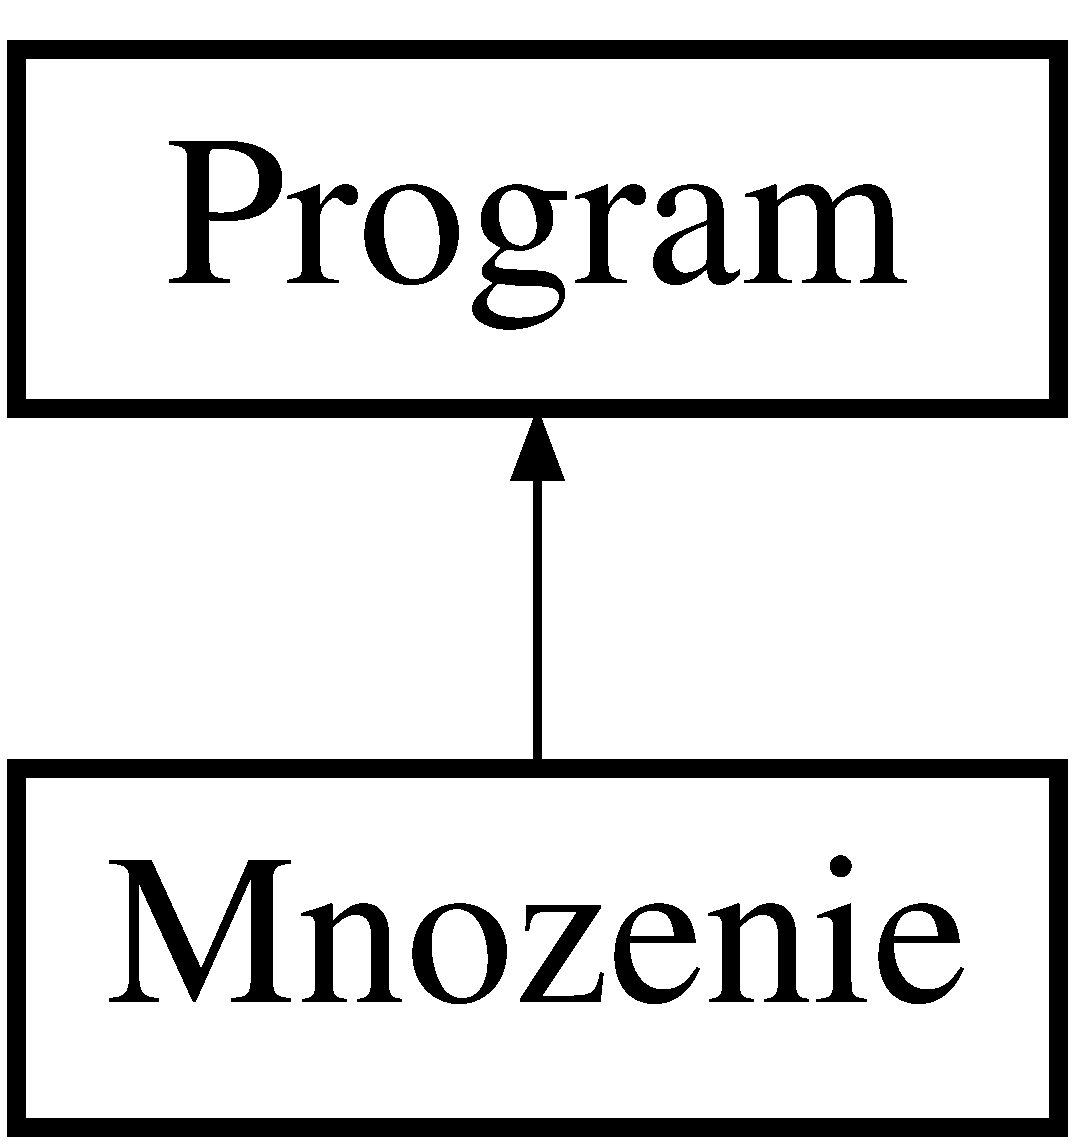
\includegraphics[height=2.000000cm]{class_mnozenie}
\end{center}
\end{figure}
\subsection*{Public Member Functions}
\begin{DoxyCompactItemize}
\item 
bool \hyperlink{class_mnozenie_a540045a41aef8f58ecbf6c9afe606d85}{wykonaj\-\_\-program} ()
\begin{DoxyCompactList}\small\item\em Metoda wykonaj\-\_\-program. \end{DoxyCompactList}\end{DoxyCompactItemize}
\subsection*{Additional Inherited Members}


\subsection{Detailed Description}
Klasa \hyperlink{class_mnozenie}{Mnozenie}. 

Klasa pochodna klasy bazowej \hyperlink{class_program}{Program} wykonujaca mnozenie danych razy dwa. 

\subsection{Member Function Documentation}
\hypertarget{class_mnozenie_a540045a41aef8f58ecbf6c9afe606d85}{\index{Mnozenie@{Mnozenie}!wykonaj\-\_\-program@{wykonaj\-\_\-program}}
\index{wykonaj\-\_\-program@{wykonaj\-\_\-program}!Mnozenie@{Mnozenie}}
\subsubsection[{wykonaj\-\_\-program}]{\setlength{\rightskip}{0pt plus 5cm}bool Mnozenie\-::wykonaj\-\_\-program (
\begin{DoxyParamCaption}
{}
\end{DoxyParamCaption}
)\hspace{0.3cm}{\ttfamily [virtual]}}}\label{class_mnozenie_a540045a41aef8f58ecbf6c9afe606d85}


Metoda wykonaj\-\_\-program. 

Metoda nadpisana na metode klasy bazowej wykonujaca algorytm zgodny z funkcja klasy. \begin{DoxyReturn}{Returns}
Zwraca wartosc true jezeli wykonano zadana operacje lub wartosc false jezeli operacja sie nie powiodla. 
\end{DoxyReturn}


Reimplemented from \hyperlink{class_program_ac396401ba5cade863d0e6acb727bec4e}{Program}.



The documentation for this class was generated from the following files\-:\begin{DoxyCompactItemize}
\item 
inc/\hyperlink{mnozenie_8hh}{mnozenie.\-hh}\item 
src/\hyperlink{mnozenie_8cpp}{mnozenie.\-cpp}\end{DoxyCompactItemize}

\hypertarget{class_program}{\section{Program Class Reference}
\label{class_program}\index{Program@{Program}}
}


Klasa \hyperlink{class_program}{Program}.  




{\ttfamily \#include $<$program.\-hh$>$}

Inheritance diagram for Program\-:\begin{figure}[H]
\begin{center}
\leavevmode
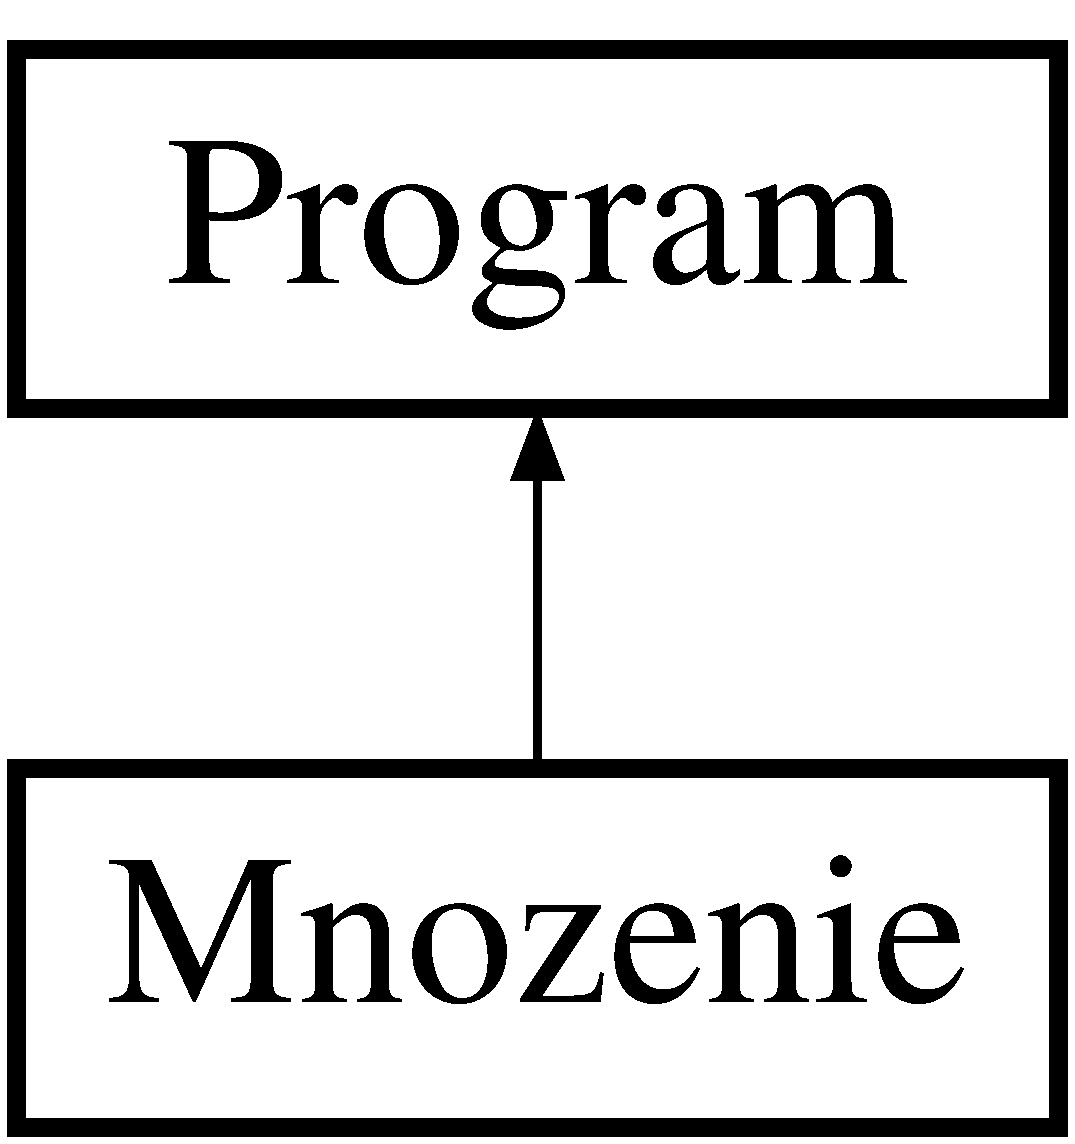
\includegraphics[height=2.000000cm]{class_program}
\end{center}
\end{figure}
\subsection*{Public Member Functions}
\begin{DoxyCompactItemize}
\item 
bool \hyperlink{class_program_aaef7fcaf64830eb231cbb9e887d705af}{zapisz\-\_\-dane} (char $\ast$nazwa)
\begin{DoxyCompactList}\small\item\em Metoda zapisz\-\_\-dane. \end{DoxyCompactList}\item 
void \hyperlink{class_program_a060ea3afebf696152d50135d20856e5a}{wypisz\-\_\-dane} ()
\begin{DoxyCompactList}\small\item\em Metoda wypisz\-\_\-dane. \end{DoxyCompactList}\item 
bool \hyperlink{class_program_ab5441e0e8ecd02ffeada4d77aaad2726}{porownaj\-\_\-dane} (char $\ast$nazwa)
\begin{DoxyCompactList}\small\item\em Metoda porownaj\-\_\-dane. \end{DoxyCompactList}\item 
virtual bool \hyperlink{class_program_ac396401ba5cade863d0e6acb727bec4e}{wykonaj\-\_\-program} ()
\begin{DoxyCompactList}\small\item\em Metoda wykonaj\-\_\-program. \end{DoxyCompactList}\item 
clock\-\_\-t \hyperlink{class_program_ab68c69977637eb8cc05a57e176a21986}{zacznij\-\_\-pomiar\-\_\-czasu} ()
\begin{DoxyCompactList}\small\item\em Metoda zacznij\-\_\-pomiar\-\_\-czasu. \end{DoxyCompactList}\item 
clock\-\_\-t \hyperlink{class_program_a3515568f8df7224bfd8fd8b7b76ab0ba}{zakoncz\-\_\-pomiar\-\_\-czasu} ()
\begin{DoxyCompactList}\small\item\em Metoda zakoncz\-\_\-pomiar\-\_\-czasu. \end{DoxyCompactList}\end{DoxyCompactItemize}
\subsection*{Public Attributes}
\begin{DoxyCompactItemize}
\item 
\hypertarget{class_program_ac27fc896de0e4c87cc6a17290c0930ef}{\hyperlink{class_tablica}{Tablica} {\bfseries dane}}\label{class_program_ac27fc896de0e4c87cc6a17290c0930ef}

\item 
clock\-\_\-t \hyperlink{class_program_a8cdcc795adc329732f41b399044d0a5b}{czas\-\_\-rozpoczecia}
\begin{DoxyCompactList}\small\item\em Zmienna czas\-\_\-rozpoczecia. \end{DoxyCompactList}\item 
fstream \hyperlink{class_program_a532ceacb1d70da66142bab96a3eb0753}{plik\-\_\-wejsciowy}
\begin{DoxyCompactList}\small\item\em Zmienna plik\-\_\-wejsciowy. \end{DoxyCompactList}\item 
fstream \hyperlink{class_program_aaa305591a4333d799c8d353f3072d8e0}{plik\-\_\-wyjsciowy}
\begin{DoxyCompactList}\small\item\em Zmienna plik\-\_\-wyjsciowy. \end{DoxyCompactList}\end{DoxyCompactItemize}


\subsection{Detailed Description}
Klasa \hyperlink{class_program}{Program}. 

Klasa odpowiedzialana za wykonanie operacji zwiazanych z pomiarem czasu oraz obsluge plikow, na ktorych wykonywane sa dzialania. Jest to klasa bazowa dla poszczegolnych algorytmow, ktorych metody moga zostac nadpisane. 

\subsection{Member Function Documentation}
\hypertarget{class_program_ab5441e0e8ecd02ffeada4d77aaad2726}{\index{Program@{Program}!porownaj\-\_\-dane@{porownaj\-\_\-dane}}
\index{porownaj\-\_\-dane@{porownaj\-\_\-dane}!Program@{Program}}
\subsubsection[{porownaj\-\_\-dane}]{\setlength{\rightskip}{0pt plus 5cm}bool Program\-::porownaj\-\_\-dane (
\begin{DoxyParamCaption}
\item[{char $\ast$}]{nazwa}
\end{DoxyParamCaption}
)}}\label{class_program_ab5441e0e8ecd02ffeada4d77aaad2726}


Metoda porownaj\-\_\-dane. 

Metoda porownujaca otrzymane dane ze spodziewanym wynikiem. 
\begin{DoxyParams}[1]{Parameters}
\mbox{\tt in}  & {\em Wskaznik} & do pliku zawierajacego poprawny wynik obliczen. \\
\hline
\end{DoxyParams}
\begin{DoxyReturn}{Returns}
Metoda zwraca wartosc true jesli udalo sie otworzyc odpowiedni plik i dane sa zgodne z wynikajacymi z obliczen. W przeciwynym wypadku metoda zwraca wartosc false i wyswietla odpowiedni komunikat. 
\end{DoxyReturn}
\hypertarget{class_program_ac396401ba5cade863d0e6acb727bec4e}{\index{Program@{Program}!wykonaj\-\_\-program@{wykonaj\-\_\-program}}
\index{wykonaj\-\_\-program@{wykonaj\-\_\-program}!Program@{Program}}
\subsubsection[{wykonaj\-\_\-program}]{\setlength{\rightskip}{0pt plus 5cm}bool Program\-::wykonaj\-\_\-program (
\begin{DoxyParamCaption}
{}
\end{DoxyParamCaption}
)\hspace{0.3cm}{\ttfamily [virtual]}}}\label{class_program_ac396401ba5cade863d0e6acb727bec4e}


Metoda wykonaj\-\_\-program. 

Metoda wykonujaca glowny algorytm programu. \begin{DoxyReturn}{Returns}
Metoda zwraca wartosc false jesli nie zostala nadpisana inna metoda z klasy dziedziczacej i wyswietla odpowiedni komunikat. 
\end{DoxyReturn}
\hypertarget{class_program_a060ea3afebf696152d50135d20856e5a}{\index{Program@{Program}!wypisz\-\_\-dane@{wypisz\-\_\-dane}}
\index{wypisz\-\_\-dane@{wypisz\-\_\-dane}!Program@{Program}}
\subsubsection[{wypisz\-\_\-dane}]{\setlength{\rightskip}{0pt plus 5cm}void Program\-::wypisz\-\_\-dane (
\begin{DoxyParamCaption}
{}
\end{DoxyParamCaption}
)}}\label{class_program_a060ea3afebf696152d50135d20856e5a}


Metoda wypisz\-\_\-dane. 

Metoda, ktora wypisuje przetworzone dane na standardowym wyjsciu. \hypertarget{class_program_ab68c69977637eb8cc05a57e176a21986}{\index{Program@{Program}!zacznij\-\_\-pomiar\-\_\-czasu@{zacznij\-\_\-pomiar\-\_\-czasu}}
\index{zacznij\-\_\-pomiar\-\_\-czasu@{zacznij\-\_\-pomiar\-\_\-czasu}!Program@{Program}}
\subsubsection[{zacznij\-\_\-pomiar\-\_\-czasu}]{\setlength{\rightskip}{0pt plus 5cm}clock\-\_\-t Program\-::zacznij\-\_\-pomiar\-\_\-czasu (
\begin{DoxyParamCaption}
{}
\end{DoxyParamCaption}
)}}\label{class_program_ab68c69977637eb8cc05a57e176a21986}


Metoda zacznij\-\_\-pomiar\-\_\-czasu. 

Metoda zapisujaca czas rozpoczecia pomiaru w odpowiednim polu klasy. \begin{DoxyReturn}{Returns}
Zwraca odczytany czas. 
\end{DoxyReturn}
\hypertarget{class_program_a3515568f8df7224bfd8fd8b7b76ab0ba}{\index{Program@{Program}!zakoncz\-\_\-pomiar\-\_\-czasu@{zakoncz\-\_\-pomiar\-\_\-czasu}}
\index{zakoncz\-\_\-pomiar\-\_\-czasu@{zakoncz\-\_\-pomiar\-\_\-czasu}!Program@{Program}}
\subsubsection[{zakoncz\-\_\-pomiar\-\_\-czasu}]{\setlength{\rightskip}{0pt plus 5cm}clock\-\_\-t Program\-::zakoncz\-\_\-pomiar\-\_\-czasu (
\begin{DoxyParamCaption}
{}
\end{DoxyParamCaption}
)}}\label{class_program_a3515568f8df7224bfd8fd8b7b76ab0ba}


Metoda zakoncz\-\_\-pomiar\-\_\-czasu. 

\begin{DoxyReturn}{Returns}
Zwraca dlugosc czasu wykonania programu (ilosc taktow zegara podzielona przez preskaler). 
\end{DoxyReturn}
\hypertarget{class_program_aaef7fcaf64830eb231cbb9e887d705af}{\index{Program@{Program}!zapisz\-\_\-dane@{zapisz\-\_\-dane}}
\index{zapisz\-\_\-dane@{zapisz\-\_\-dane}!Program@{Program}}
\subsubsection[{zapisz\-\_\-dane}]{\setlength{\rightskip}{0pt plus 5cm}bool Program\-::zapisz\-\_\-dane (
\begin{DoxyParamCaption}
\item[{char $\ast$}]{nazwa}
\end{DoxyParamCaption}
)}}\label{class_program_aaef7fcaf64830eb231cbb9e887d705af}


Metoda zapisz\-\_\-dane. 


\begin{DoxyParams}[1]{Parameters}
\mbox{\tt in}  & {\em Wskaznik} & do nazwy pliku, pod ktorym ma zostac zapisany strumien wyjsciowy. \\
\hline
\end{DoxyParams}
\begin{DoxyReturn}{Returns}
Zwraca 
\end{DoxyReturn}


\subsection{Member Data Documentation}
\hypertarget{class_program_a8cdcc795adc329732f41b399044d0a5b}{\index{Program@{Program}!czas\-\_\-rozpoczecia@{czas\-\_\-rozpoczecia}}
\index{czas\-\_\-rozpoczecia@{czas\-\_\-rozpoczecia}!Program@{Program}}
\subsubsection[{czas\-\_\-rozpoczecia}]{\setlength{\rightskip}{0pt plus 5cm}clock\-\_\-t Program\-::czas\-\_\-rozpoczecia}}\label{class_program_a8cdcc795adc329732f41b399044d0a5b}


Zmienna czas\-\_\-rozpoczecia. 

Zawiera czas w ktorym zaczal wykonywac sie wlasciwy kod algorytmu (liczony od momentu uruchomienia programu). Do tej danej porownywany jest czas zakoczenia wykonywania algorytmu. \hypertarget{class_program_a532ceacb1d70da66142bab96a3eb0753}{\index{Program@{Program}!plik\-\_\-wejsciowy@{plik\-\_\-wejsciowy}}
\index{plik\-\_\-wejsciowy@{plik\-\_\-wejsciowy}!Program@{Program}}
\subsubsection[{plik\-\_\-wejsciowy}]{\setlength{\rightskip}{0pt plus 5cm}fstream Program\-::plik\-\_\-wejsciowy}}\label{class_program_a532ceacb1d70da66142bab96a3eb0753}


Zmienna plik\-\_\-wejsciowy. 

Zmienna przedstawiajaca otwarty plik jako strumien danych. \hypertarget{class_program_aaa305591a4333d799c8d353f3072d8e0}{\index{Program@{Program}!plik\-\_\-wyjsciowy@{plik\-\_\-wyjsciowy}}
\index{plik\-\_\-wyjsciowy@{plik\-\_\-wyjsciowy}!Program@{Program}}
\subsubsection[{plik\-\_\-wyjsciowy}]{\setlength{\rightskip}{0pt plus 5cm}fstream Program\-::plik\-\_\-wyjsciowy}}\label{class_program_aaa305591a4333d799c8d353f3072d8e0}


Zmienna plik\-\_\-wyjsciowy. 

Zmienna przedstawiajaca strumien danych po wykonaniu wlasiwego algorytmu. 

The documentation for this class was generated from the following files\-:\begin{DoxyCompactItemize}
\item 
inc/\hyperlink{program_8hh}{program.\-hh}\item 
src/\hyperlink{program_8cpp}{program.\-cpp}\end{DoxyCompactItemize}

\chapter{File Documentation}
\hypertarget{benchmark_8hh}{\section{inc/benchmark.hh File Reference}
\label{benchmark_8hh}\index{inc/benchmark.\-hh@{inc/benchmark.\-hh}}
}


Plik zawierajacy deklaracje klasy benchmark.  


{\ttfamily \#include \char`\"{}program.\-hh\char`\"{}}\\*
\subsection*{Classes}
\begin{DoxyCompactItemize}
\item 
class \hyperlink{classbenchmark}{benchmark}
\begin{DoxyCompactList}\small\item\em Klasa benchmarek. \end{DoxyCompactList}\end{DoxyCompactItemize}


\subsection{Detailed Description}
Plik zawierajacy deklaracje klasy benchmark. 
\hypertarget{mnozenie_8hh}{\section{inc/mnozenie.hh File Reference}
\label{mnozenie_8hh}\index{inc/mnozenie.\-hh@{inc/mnozenie.\-hh}}
}


Plik zawierajacy deklaracje klasy \hyperlink{class_mnozenie}{Mnozenie}.  


{\ttfamily \#include \char`\"{}program.\-hh\char`\"{}}\\*
\subsection*{Classes}
\begin{DoxyCompactItemize}
\item 
class \hyperlink{class_mnozenie}{Mnozenie}
\begin{DoxyCompactList}\small\item\em Klasa \hyperlink{class_mnozenie}{Mnozenie}. \end{DoxyCompactList}\end{DoxyCompactItemize}


\subsection{Detailed Description}
Plik zawierajacy deklaracje klasy \hyperlink{class_mnozenie}{Mnozenie}. 
\hypertarget{program_8hh}{\section{inc/program.hh File Reference}
\label{program_8hh}\index{inc/program.\+hh@{inc/program.\+hh}}
}


Plik zawierajacy deklaracje klasy \hyperlink{class_program}{Program}.  


{\ttfamily \#include $<$fstream$>$}\\*
{\ttfamily \#include $<$ctime$>$}\\*
{\ttfamily \#include $<$cstdio$>$}\\*
{\ttfamily \#include \char`\"{}tablica.\+hh\char`\"{}}\\*
\subsection*{Classes}
\begin{DoxyCompactItemize}
\item 
class \hyperlink{class_program}{Program}
\begin{DoxyCompactList}\small\item\em Klasa \hyperlink{class_program}{Program}. \end{DoxyCompactList}\end{DoxyCompactItemize}


\subsection{Detailed Description}
Plik zawierajacy deklaracje klasy \hyperlink{class_program}{Program}. 


\hypertarget{benchmark_8cpp}{\section{src/benchmark.cpp File Reference}
\label{benchmark_8cpp}\index{src/benchmark.\+cpp@{src/benchmark.\+cpp}}
}


Plik zawierajacy definicje metod klasy benchmark.  


{\ttfamily \#include $<$iostream$>$}\\*
{\ttfamily \#include $<$ctime$>$}\\*
{\ttfamily \#include $<$cstdlib$>$}\\*
{\ttfamily \#include $<$string$>$}\\*
{\ttfamily \#include $<$sstream$>$}\\*
{\ttfamily \#include \char`\"{}przykladowy\+\_\+program.\+hh\char`\"{}}\\*
{\ttfamily \#include \char`\"{}benchmark.\+hh\char`\"{}}\\*
{\ttfamily \#include \char`\"{}komunikacja.\+hh\char`\"{}}\\*
{\ttfamily \#include \char`\"{}konfiguracja.\+hh\char`\"{}}\\*
{\ttfamily \#include \char`\"{}tab\+\_\+hash.\+hh\char`\"{}}\\*
{\ttfamily \#include \char`\"{}element.\+hh\char`\"{}}\\*


\subsection{Detailed Description}
Plik zawierajacy definicje metod klasy benchmark. 


\hypertarget{main_8cpp}{\section{src/main.cpp File Reference}
\label{main_8cpp}\index{src/main.\+cpp@{src/main.\+cpp}}
}


Plik zawierajacy glowna funkcje programu wykonujacego benchmark algorytmu.  


{\ttfamily \#include $<$iostream$>$}\\*
{\ttfamily \#include \char`\"{}komunikacja.\+hh\char`\"{}}\\*
{\ttfamily \#include \char`\"{}benchmark.\+hh\char`\"{}}\\*
\subsection*{Functions}
\begin{DoxyCompactItemize}
\item 
int \hyperlink{main_8cpp_a840291bc02cba5474a4cb46a9b9566fe}{main} (void)
\begin{DoxyCompactList}\small\item\em Glowna funkcja programu. \end{DoxyCompactList}\end{DoxyCompactItemize}


\subsection{Detailed Description}
Plik zawierajacy glowna funkcje programu wykonujacego benchmark algorytmu. 



\subsection{Function Documentation}
\hypertarget{main_8cpp_a840291bc02cba5474a4cb46a9b9566fe}{\index{main.\+cpp@{main.\+cpp}!main@{main}}
\index{main@{main}!main.\+cpp@{main.\+cpp}}
\subsubsection[{main}]{\setlength{\rightskip}{0pt plus 5cm}int main (
\begin{DoxyParamCaption}
\item[{void}]{}
\end{DoxyParamCaption}
)}}\label{main_8cpp_a840291bc02cba5474a4cb46a9b9566fe}


Glowna funkcja programu. 

Funkcja wykonujaca benchmark zadanego algorytmu na podstawie czasu wykonywania operacji. 
\hypertarget{mnozenie_8cpp}{\section{src/mnozenie.cpp File Reference}
\label{mnozenie_8cpp}\index{src/mnozenie.\-cpp@{src/mnozenie.\-cpp}}
}


Plik zawierajacy definicje metod klasy \hyperlink{class_mnozenie}{Mnozenie}.  


{\ttfamily \#include \char`\"{}mnozenie.\-hh\char`\"{}}\\*


\subsection{Detailed Description}
Plik zawierajacy definicje metod klasy \hyperlink{class_mnozenie}{Mnozenie}. 
\hypertarget{program_8cpp}{\section{src/program.cpp File Reference}
\label{program_8cpp}\index{src/program.\-cpp@{src/program.\-cpp}}
}


Plik zawierajacy definicje metod klasy \hyperlink{class_program}{Program}.  


{\ttfamily \#include $<$fstream$>$}\\*
{\ttfamily \#include $<$iostream$>$}\\*
{\ttfamily \#include $<$sstream$>$}\\*
{\ttfamily \#include $<$string$>$}\\*
{\ttfamily \#include $<$cstdio$>$}\\*
{\ttfamily \#include $<$ctime$>$}\\*
{\ttfamily \#include \char`\"{}program.\-hh\char`\"{}}\\*
{\ttfamily \#include \char`\"{}operacje.\-hh\char`\"{}}\\*
{\ttfamily \#include \char`\"{}komunikacja.\-hh\char`\"{}}\\*


\subsection{Detailed Description}
Plik zawierajacy definicje metod klasy \hyperlink{class_program}{Program}. 
%--- End generated contents ---

% Index
\newpage
\phantomsection
\addcontentsline{toc}{chapter}{Index}
\printindex

\end{document}
